%********************************************************************
% Appendix
%*******************************************************
% If problems with the headers: get headings in appendix etc. right
%\markboth{\spacedlowsmallcaps{Appendix}}{\spacedlowsmallcaps{Appendix}}
\chapter{Appendix}
\begin{figure}
\centering
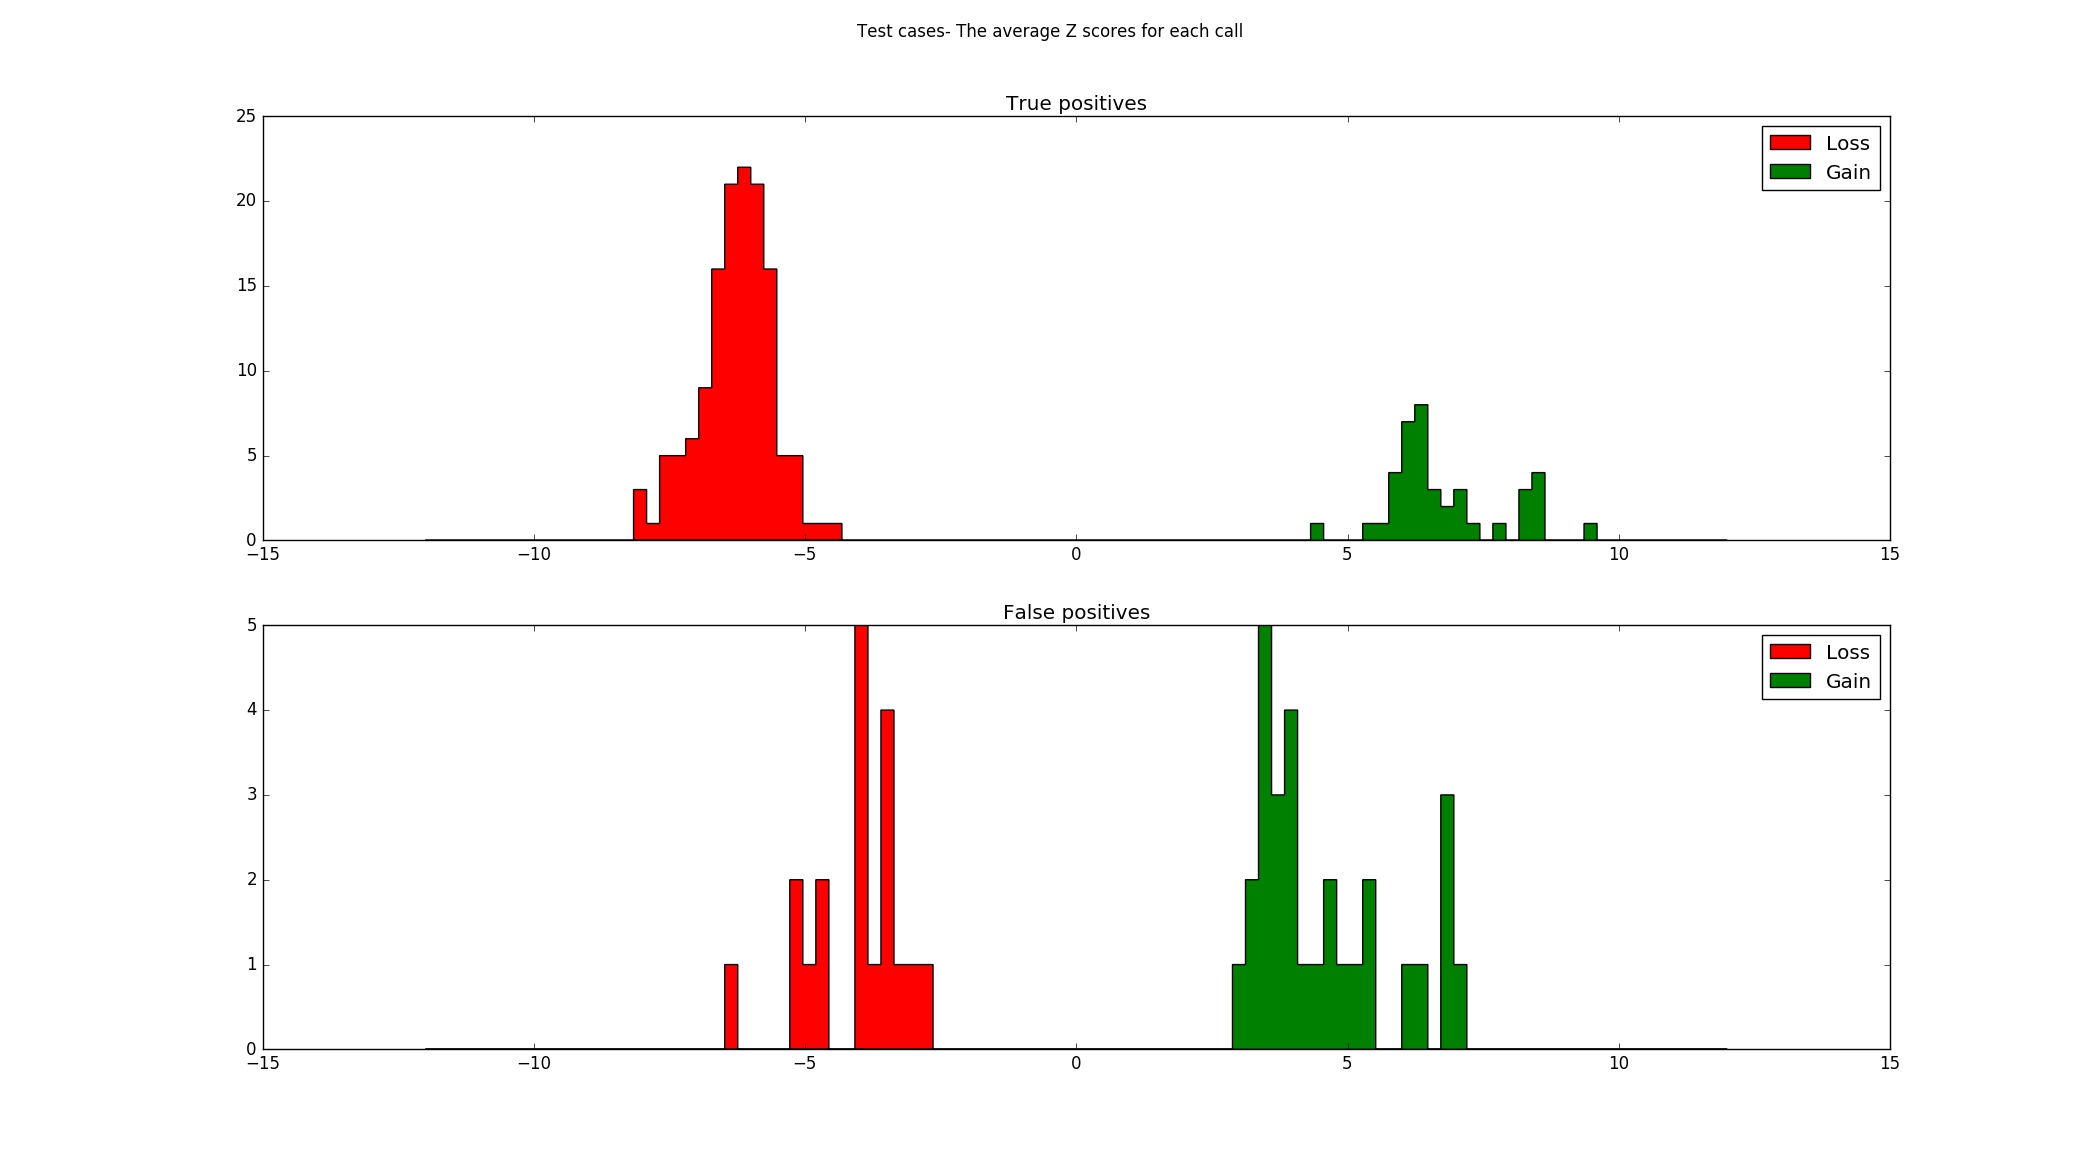
\includegraphics[width=1\linewidth]{./Figures/testcasesaverageconfidenceZscore}
\caption[Test cases: The average Z score at a threshold of 2.374]{Test cases: The average Z score in true positive calls made at a threshold of 2.374 are more significant in true positive calls than false positive calls however there is overlap between the two groups}
\label{fig:testcasesaverageconfidenceZscore}
\end{figure}

\begin{figure}
\centering
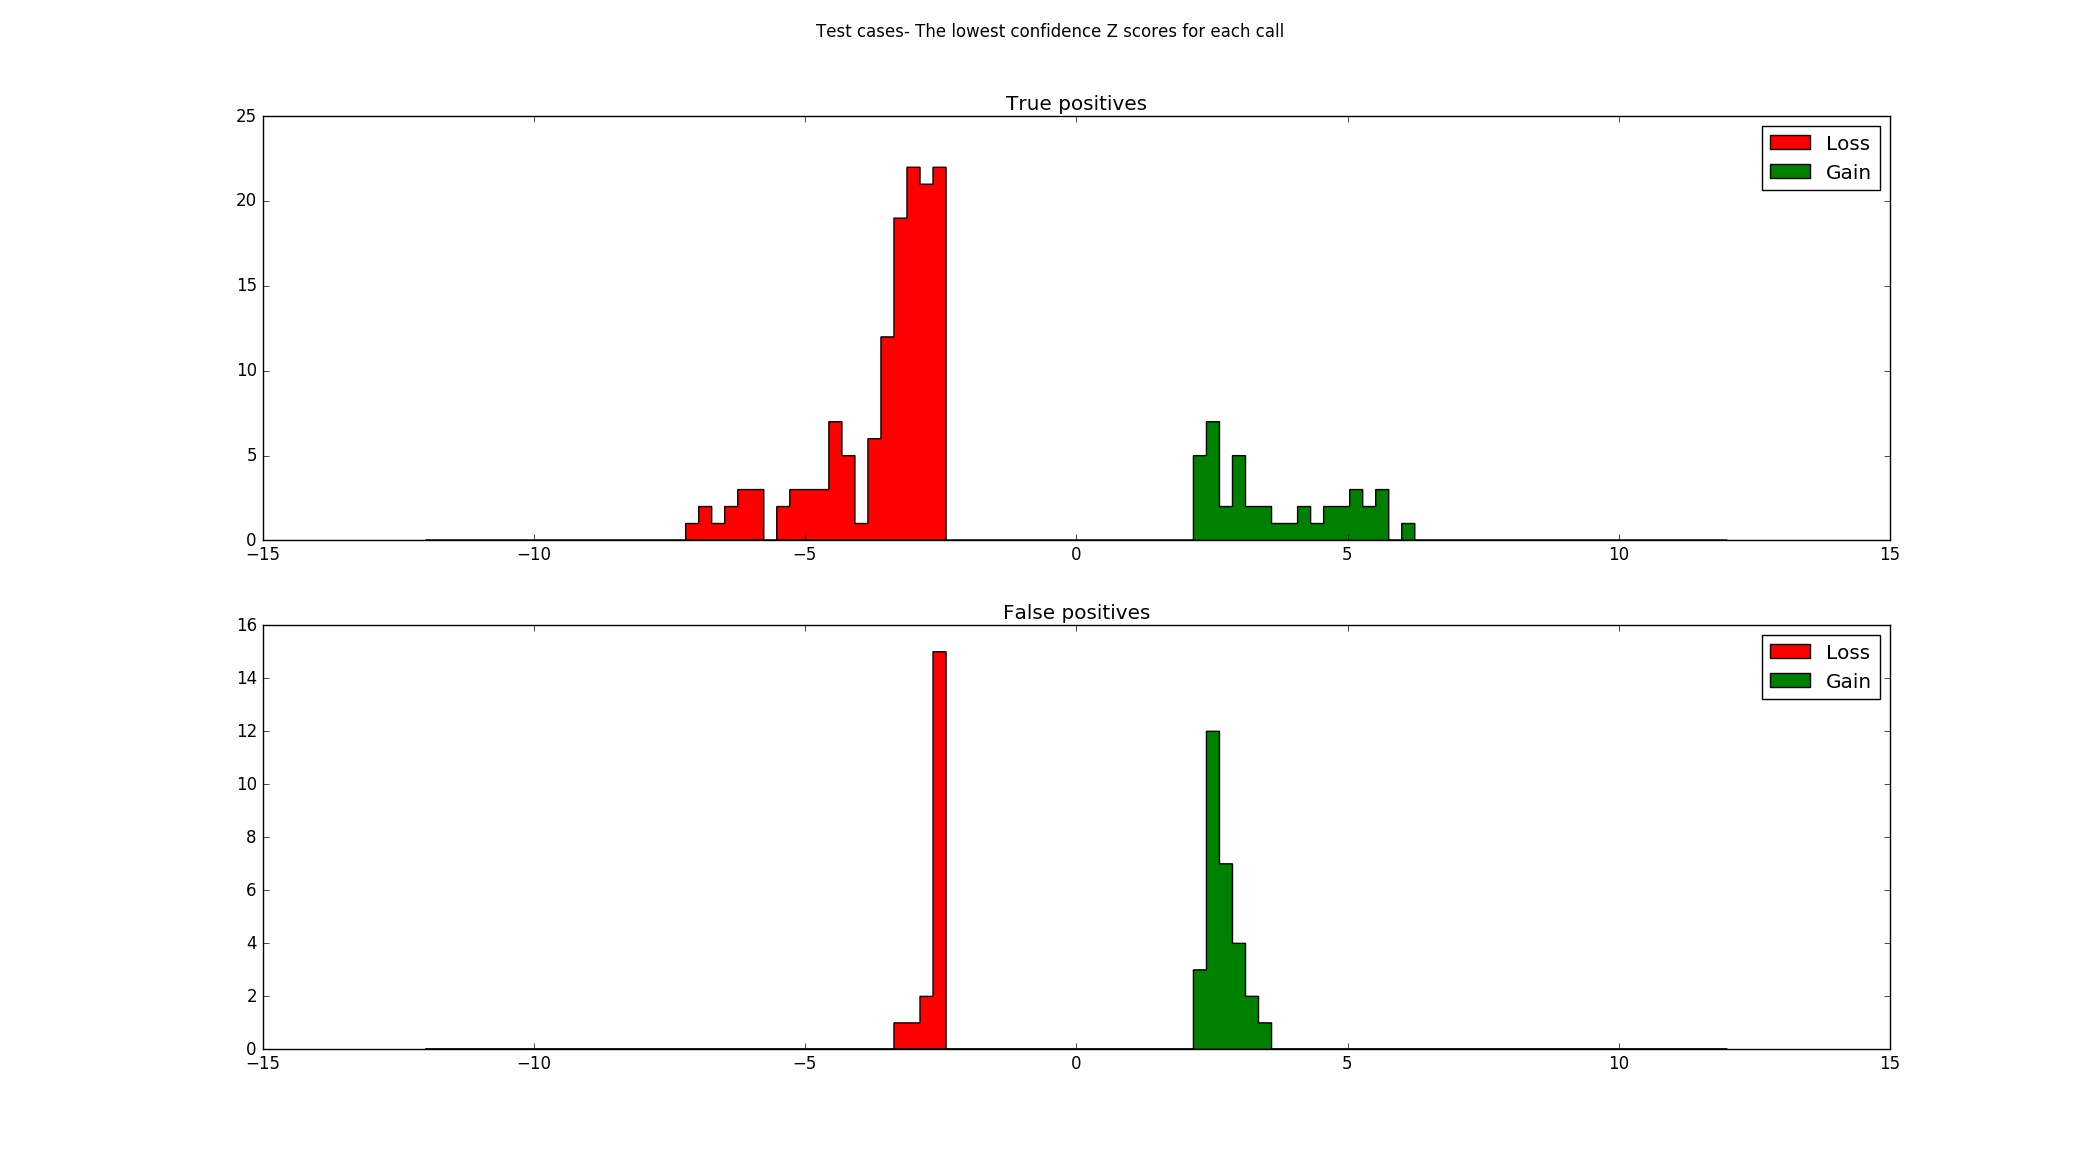
\includegraphics[width=1\linewidth]{./Figures/testcaseslowestconfidenceZscore}
\caption[Test cases: The lowest confidence probe within calls at a threshold of 2.374]{Test cases: There is overlap between the lowest confidence probe within true and false positive calls made at a threshold of 2.374}
\label{fig:testcaseslowestconfidenceZscore}
\end{figure}

\begin{figure}
\centering
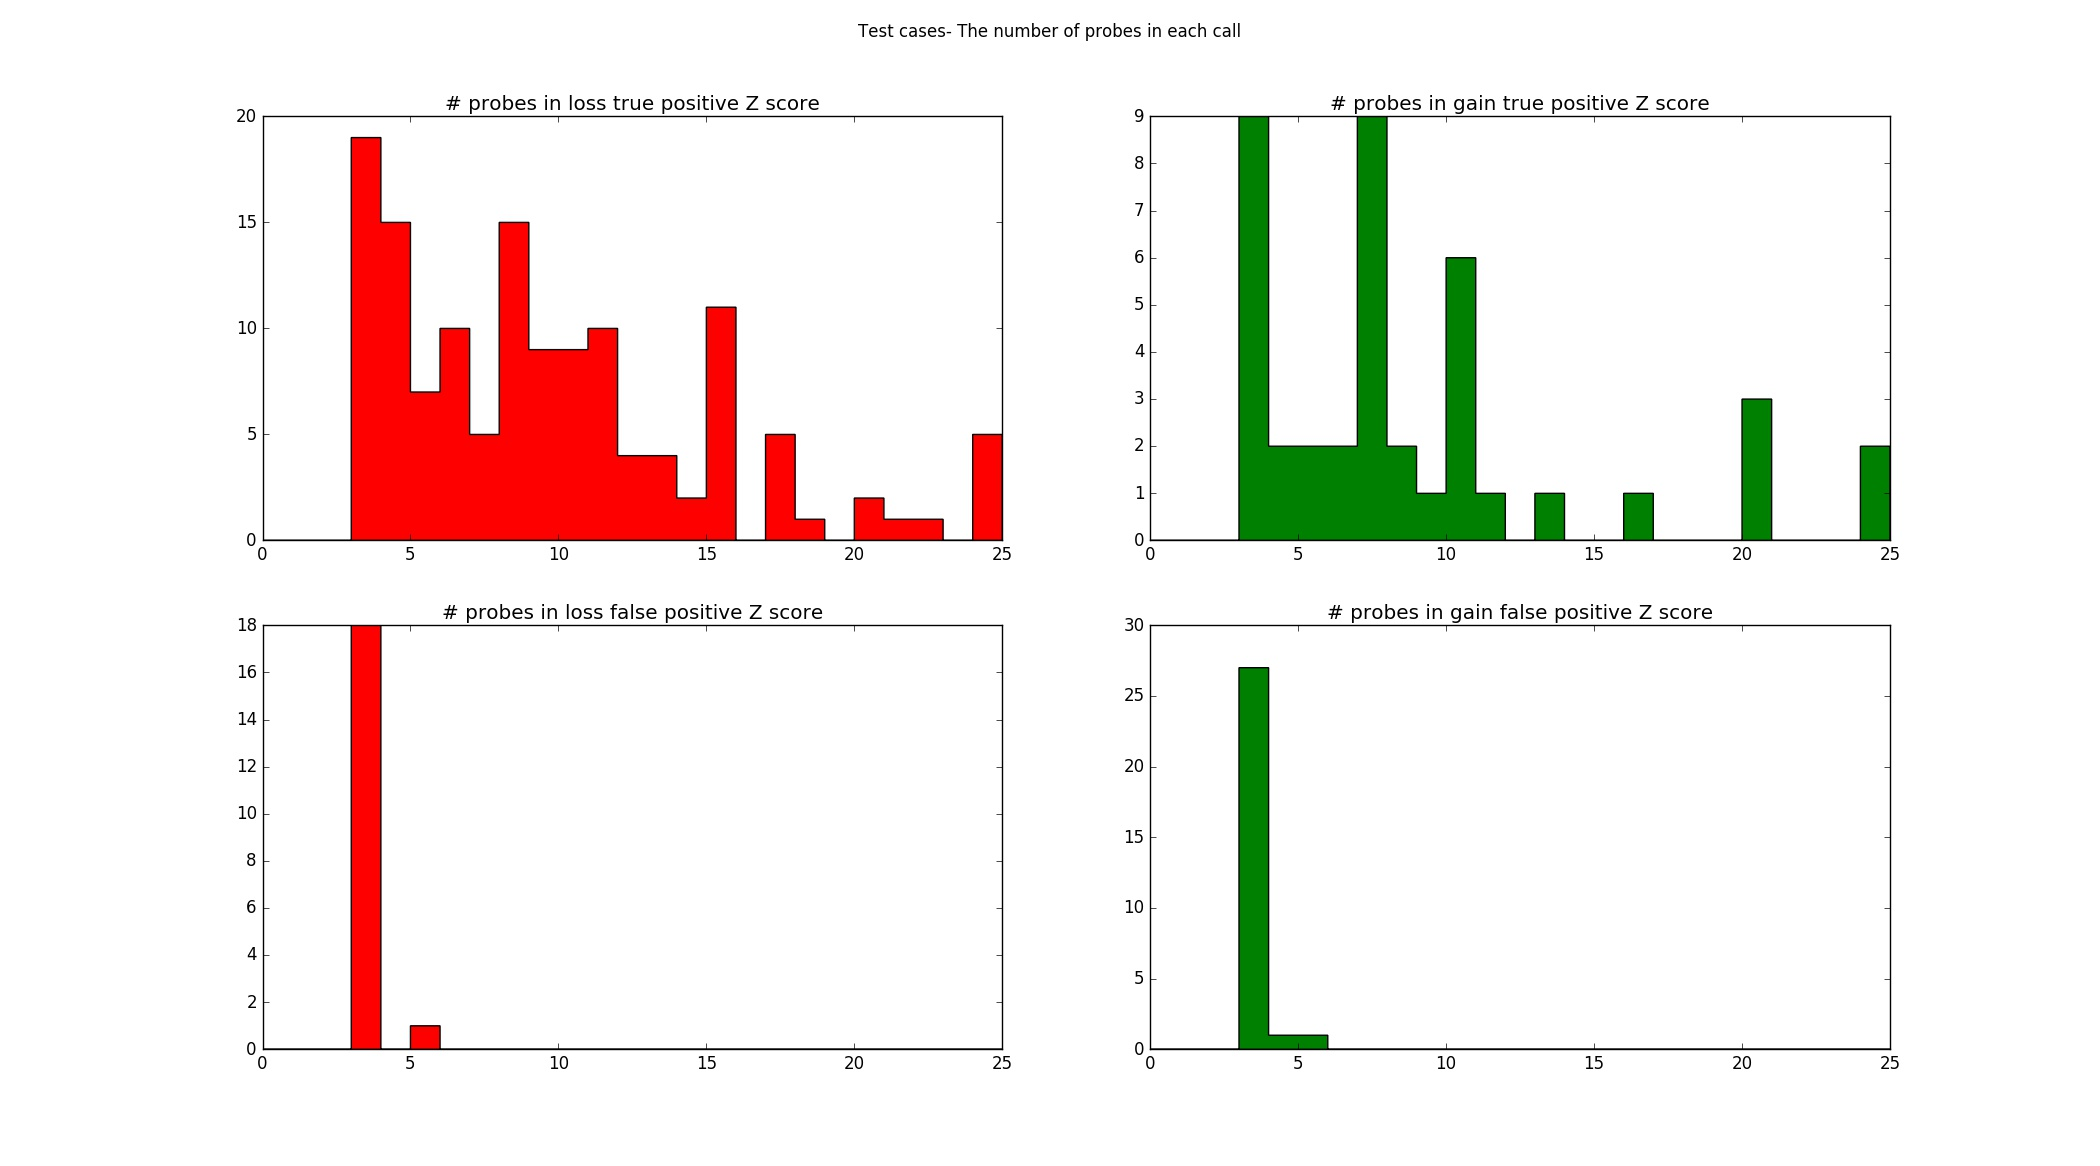
\includegraphics[width=1\linewidth]{./Figures/testcasesprobecount}
\caption[Test cases: The number of probes within calls made at a threshold of 2.374]{Test cases: At a threshold 2.374 true positive calls contain more probes than false positive calls.}
\label{fig:testcasesprobecount}
\end{figure}

\begin{figure}
\centering
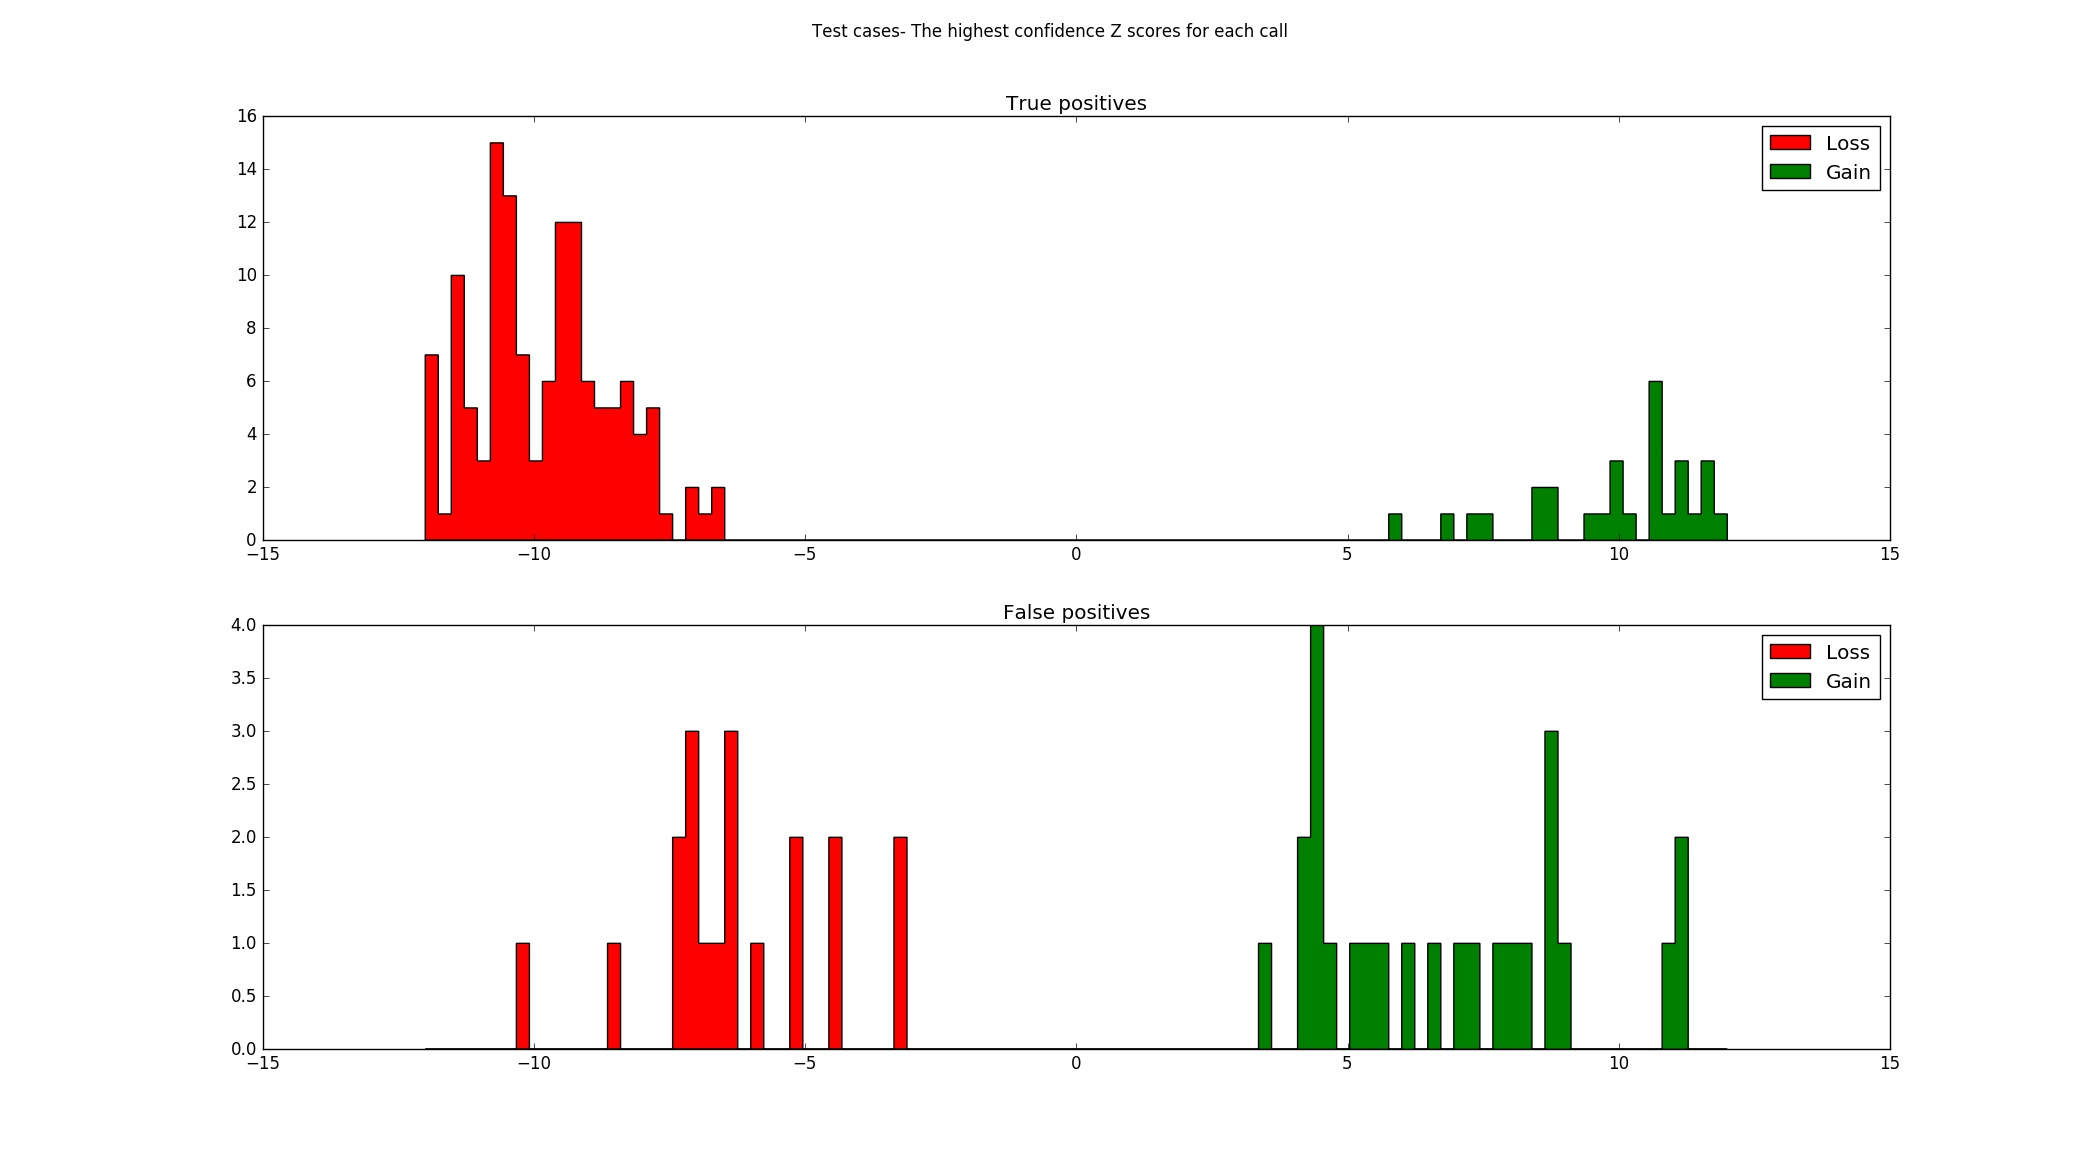
\includegraphics[width=1\linewidth]{./Figures/testcaseshighestconfidenceZscore}
\caption[Test cases: The highest confidence probe within calls made at a threshold of 2.374]{Test cases: At a Z score threshold of 2.374 there is an overlap between the highest confidence probe within true and false positive calls.}
\label{fig:testcaseshighestconfidenceZscore}
\end{figure}


\section{Further analysis of the low coverage of the 750 probe deletion on chromosome 22}\label{ch:analysisof22del}
At a threshold of 3.55 all calls from samples with the chromosome 22 deletion were made within the 73 probe region (Table  \ref{tab:chr22delcalls}).


\begin{table}[h]
\centering
\caption[Test cases: The calls made on the arrays made from the cases with the 750 probe deletion on chromosome 22]{Test cases: At a threshold of 3.55 all calls made on the arrays made from the cases with the 750 probe deletion on chromosome 22 were within a 73 probe section (probes 39733 to 39805). Of these 73 probes between 17\% and 74\% were covered by a call.}
\label{tab:chr22delcalls}
\begin{tabular}{@{}llll@{}}
\toprule
Array\_ID & first called probe & last called probe & \% of 73 probes covered (n) \\ \midrule
63        & 39735              & 39805             & 72.6 (53)                   \\
64        & 39733              & 39797             & 64.4 (47)                   \\
65        & 39735              & 39803             & 52.1 (38)                   \\
66        & 39735              & 39803             & 74 (54)                     \\
67        & 39745              & 39784             & 23.3 (17)                   \\
68        & 39745              & 39784             & 23.3 (17)                   \\
69        & 39745              & 39784             & 23.3 (17)                   \\
70        & 39743              & 39803             & 17.8 (13)                   \\ \bottomrule
\end{tabular}
\end{table}